
本文在概述原文时,着重介绍数据结构的设计。对于原文中涉及的大量引理(Lemma)、定理(Theorem)、命题(Proposition)、
推论(Corollary),本文直接引用其中的结论,不再关注其证明过程,因为原文提供了详尽的证明或证明所在的参考文献。
由于原文中直接引用了一些不太常用的数据结构,如后缀树、van Emde Boas树等,本文会适当补充相关数据结构的定义、实现、性质。
对于原文中定义不够明确的概念,本文给出了严格的定义,并描述和论证了相关性质。

\subsection{问题引入}\label{subsec:intro}

\begin{description}
    \item[MUPS] 给定串$T$,$1 \leq i \leq j \leq ||T||$,回文子串$u = T[i..j]$,如果$u$在$T$中是唯一的,
    $u^{\prime} = T[i + 1..j - 1]$在$T$中不唯一,则称$u$是$T$的极小唯一回文子串(minimal unique palindromic substring).
    \item[interval SUPS] 给定串$T$和区间$[p,q]$,回文子串$v = T[i..j]$,$v$在$T$中唯一且包含区间$[p,q]$,
    任何更短的包含区间$[p,q]$的$T$的回文子串都在$T$中不唯一,则称$v$是对区间$[p,q]$的$T$的最短唯一回文子串
    (shortest unique palindromic substring),记作$v = \mathrm{SUPS}_T ([p,q])$.
    \item[point SUPS] 区间SUPS问题在$p = q$的情况下退化为点的SUPS问题,记作$v = \mathrm{SUPS}_T (p)$.
    \item[ME] MUPS向外扩展,即每次起点向前移动一位,终点向后移动一位,直至破坏回文性为止。
    在此过程中可以得到“极小唯一回文子串的极大扩展”(maximal extension of MUPS).
    \item[MP] 对任意一个半整数,即1, 1.5, 2, 2.5 .. , n \footnote{原文中串从1开始标号,本文也采用这种规范。},
    都能求得以其为中心的极大回文子串(maximal palindrome).
\end{description}

需要注意的是,MUPS是极小的,强调的是MUPS都无法在自身基础上再缩小一点,因为再缩小会违背MUPS的唯一性,
MUPS的定义并不关心每个MUPS与其他MUPS的长度比较。SUPS是最短的,SUPS的定义基于多个包含给定区间或点的回文子串的长度比较,
但这并不意味着SUPS仅有1个。原文中的Theorem 1说明SUPS至多只有4个。

由MUPS的定义可知,MUPS具有唯一性,此外MUPS不存在嵌套的情况,可用反证法论证如下:

取MUPS $M_1 = T[s_1..e_1]$,MUPS $M_2 = [s_2..e_2]$,满足$s_1 \leq s_2 \leq e_1 \leq e_2 $,
且$s_1 \leq s_2$和$e_1 \leq e_2$不能同时取等。找到$M_1$的对称轴$l$,若$M_2$关于$l$对称,则$M_1$显然不满足MUPS定义中的极小性;
若$M_2$不关于$l$对称,则取串$M_3$关于轴$l$与$M_2$对称,由于$M_2$是回文串,$M_3$与$M_2$完全一致,显然违背了$M_2$作为MUPS的唯一性。

原文中使用的“极大回文子串”(maximal palindrome)一词,其实兼指ME和MP。这里明确地区分了这两个概念,并在下文探讨两者的性质和联系。

ME具有唯一性和非嵌套性,可用反证法论证如下:

假设存在两个完全一致的ME $m_1$和$m_2$,$m_1$对应的MUPS为$M_1$,以$m_1$和$M_1$的相对位置关系在$m_2$中找到回文子串$M_2$,
$M_2$一定与$M_1$不重合,于是违背了$M_1$作为SUPS的唯一性。ME的唯一性得证。

取ME $m_1 = T[s_1..e_1]$,ME $m_2 = [s_2..e_2]$,满足$s_1 \leq s_2 \leq e_1 \leq e_2 $,
且$s_1 \leq s_2$和$e_1 \leq e_2$不能同时取等。找到$m_1$的对称轴$l$,若$m_2$关于$l$对称,则$m_2$不满足ME定义中的极大性;
若$m_2$不关于$l$对称,则取串$m_3$关于轴$l$与$m_2$对称,由于$m_2$是回文串,$m_3$与$m_2$完全一致,
$m_2$不满足上文已证的ME的唯一性。ME的非嵌套性得证。

显然,MP完全包含了ME。通常情况下,MP包含了大量的空串和单字符串,并有大量重复情况。例如,串$T = \mathrm{babbbabbababb}$,
以2为中心的MP $\mathrm{bab}$和以11为中心的MP $\mathrm{bab}$发生重复,因此两者都不包含在ME中。

事实上,唯一且非空的MP等同于ME。证明如下:

对任意非空的MP,定义“缩小串集”为MP缩小\footnote{类似于扩展,缩小指每次将回文串的起点向后移动一位,终点向前移动一位。}过程中产生的所有回文串的总和。
易知,“缩小串集”包含了所有回文子串,也就包含了所有ME。不唯一的MP缩小产生的回文串也是不唯一的,因而不能产生ME。对唯一的MP进行缩小,缩小的尽头是空串,
必然丧失唯一性。因此,在缩小的过程中一定存在唯一性发生改变的临界,即可找到一个MUPS,则该唯一的MP也就成为一个ME。综上,唯一且非空的MP与ME一一对应。

\subsubsection{最长公共扩展(LCE)与后缀树(suffix tree)}\label{subsubsec:lce}

对于长度为$n$的串$S$,后缀树(suffix tree)定义为这样一棵树,满足如下五个条件\footnote{后缀树的定义和图\ref{fig:suffix}引自Suffix tree \textit{Wikipedia},可参见https://en.wikipedia.org/wiki/Suffix\_tree}:
\begin{itemize}
    \item 有$n$个子节点,分别编号$1$至$n$
    \item 除根节点外,每个非叶节点都有至少两个子节点
    \item 每条边都用$S$的一个非空子串来标记
    \item 起始于同一节点的两条边不能有同一字符开头的标记
    \item 从根节点到叶节点$i$,将所有边的标记依次拼接起来,可得到后缀$S[i..n]$
\end{itemize}

\begin{figure}[h]
    \centering
    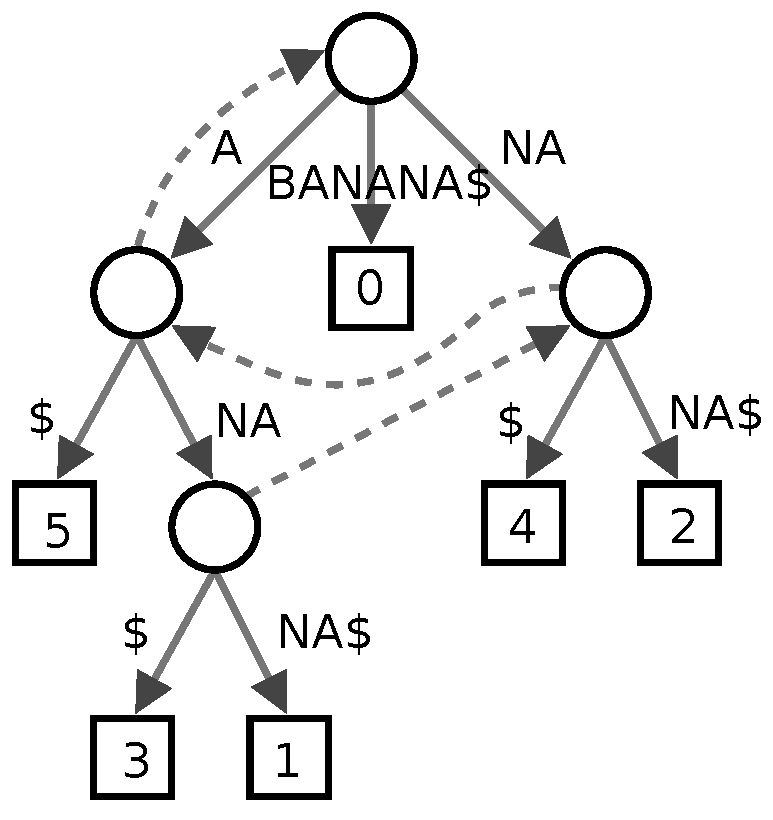
\includegraphics[width=0.8\textwidth]{resources/fig/Suffix_tree_BANANA}
    \caption{$\mathrm{BANANA\$}$的后缀树,虚线为构建过程中的辅助线}\label{fig:suffix}
\end{figure}

最长公共扩展(longest common extension, LCE)问题是对一个给定的串$T$,给定的整数$i,j$,满足$1 \leq i,j \leq n$,
计算出两个后缀$T[i..n]$和$T[j..n]$的最长公共前缀的长度。LCE问题可以通过构建串$T\$$\footnote{这里的\$,图\ref{fig:suffix}中的\$,以及下文出现的\#,都指不属于字母表$\Sigma$的特殊字符。}
的后缀树\footnote{解决某一问题的常用数据结构可用问题名代指。例如,这里的数据结构可称为LCE数据结构。}在常数时间内求得\cite{Gusfield_1997}。我们可以构造一个双向LCE数据结构,即对串$T\#T^R\$$构造后缀树,从而实现在常数时间内求得:
\begin{itemize}
    \item $T$的任意两后缀的最长公共前缀
    \item $T$的任意两前缀的逆的最长公共前缀
    \item $T$的任意后缀和$T$的任意前缀的逆的最长公共前缀
\end{itemize}
由第三点易知,对任意位$c$,将$T$分割为前缀$T_1$和后缀$T_2$,我们可以用双向LCE数据结构求得$T_2$和$T_1^R$的最长公共前缀,即以$c$为中心的极大回文子串。

\subsubsection{区域最小值请求(RmQ)及其变体LogRmQ}\label{subsubsec:rmq}

区域最小值请求(range minimum query, RmQ)是对一个给定的整型数组$A$,$A$上的两个下标$i,j$,满足$i \leq j$,
计算出下标$k$使得$A[k]$为$A[i..j]$上的最小值。需要注意的是,有时最小值有多个,而RmQ每次只能找到其中一个。
存在这样一个数据结构,可以在$O(n)$时间内构建,并在$O(1)$时间内回应任一个RmQ。

对于一个RmQ,如果任何请求的范围宽度都满足$O(\mathrm{polylog}(n))$,则称这样的RmQ为LogRmQ。

\subsection{前驱(predecessor)、后继(successor)与van Emde Boas树}\label{subsec:van}

对一个不减的整型数组$B$,给定整型数$x$,定义前驱(predecessor)是小于$x$的最大值;同理,定义后继(successor)是大于$x$的最小值。
我们使用van Emde Boas树求解前驱和后继。van Emde Boas树的空间复杂度为$O(U)$,各项操作的时间复杂度为$O(\log\log U)$,
其中$U$为全局大小(universal size)\cite{Cormen3ed}。在回文串领域,取$U = n$.

\subsection{Inoue算法概述}\label{subsec:inoue}

Inoue算法\cite{Inoue2018}的数据结构由下面五部分组成:
\begin{itemize}
    \item 所有MUPS的集合
    \item 所有MP的集合
    \item 对所有MUPS开始位置组成的数组求后继的数据结构
    \item 对所有MUPS结束位置组成的数组求前驱的数据结构
    \item 所有MUPS的长度,按照MUPS的开始位置排序,组成的数组$\mathrm{MUPSlen}$,以及对该数组的RmQ数据结构
\end{itemize}

对给定的区间$[p,q]$,通过分别对相应数组求$p$的前驱和$q$的后继,考察区间$[p,q]$覆盖MUPS的情况:
\begin{enumerate}
    \item $[p,q]$只覆盖1个MUPS,则该MUPS的能覆盖区间$[p,q]$的最小扩展即为所求。
    \item $[p,q]$覆盖多个MUPS,则无解,因为任何SUPS最多只能包含一个MUPS\cite{Inoue2018}。
    \item 找不到这样的MUPS,再分为如下三种情况。
\end{enumerate}

\begin{enumerate}
    \item 基于$q$前结束的最右边的MUPS $M_l$的扩展
    \item 一个覆盖$[p,q]$的MUPS
    \item 基于$p$前开始的最左边的MUPS $M_r$的扩展
\end{enumerate}
依次分析求解即可。其中要利用所有MP的集合求解特定中心的MP,以及递归地使用RmQ以求出所有SUPS。所有MP的集合和所有MUPS的集合可在$O(n)$时间内求得\cite{Inoue2018,Manacher75},
同时可构造完相应的前驱、后继、RmQ数据结构,且该算法数据结构五部分的空间复杂度都为$O(n)$,所以总的来说,空间复杂度为$O(n)$,预处理的时间复杂度为$O(n)$.
设共有满足条件的SUPS $\alpha$个,该算法中各个元操作的时间复杂度都为$O(1)$,且$\alpha$决定了最后RmQ递归搜索的次数,所以该算法求解SUPS问题的时间复杂度为$O(\alpha)$.

\subsection{原文对Inoue算法的改进}\label{subsec:progress}

原文对Inoue算法的改进可总结为如下几个方面:
\begin{itemize}
    \item 不再保留所有MP的集合,而是使用\ref{subsubsec:lce}中的双向LCE数据结构求解特定中心的MP。但仍需$O(n)$的空间和$O(n)$时间预处理。
    \item 使用位数组\footnote{只有0和1两种元素的数组,类似于Java中的boolean型数组。}$B, E, L$分别保存MUPS的起点、MUPS的终点、ME的起点。
    ME的终点不需要保存,因为ME和MUPS一一对应,可由MUPS的终点和MUPS起点与ME起点之差计算出ME的终点。但仍需$O(n)$的空间和$O(n)$时间预处理。
    \item 证明不等式$|\mathrm{SUPS}_T ([p,q])| \leq 4$恒成立(原文中的Theorem 1),即$\alpha \leq 4$,故$O(\alpha) = O(1)$.
\end{itemize}

\subsection{原文算法的示例}\label{subsec:example}

可参见原文Fig.6。
